\documentclass[english]{article}
\usepackage[utf8x]{inputenc}
\usepackage[T1]{fontenc}
\usepackage{babel}
\usepackage{amsmath}
\usepackage{graphicx}
\usepackage{fancyhdr}
\usepackage[numbers]{natbib}
\usepackage{subcaption}
\pagestyle{fancy}
\fancyhf{}
\renewcommand{\headrulewidth}{0pt}
\setlength{\headheight}{40pt} 
\usepackage[a4paper,top=3cm,bottom=2cm,left=3cm,right=3cm,marginparwidth=1.75cm]{geometry}

\begin{document}


\title{\bf Analysing and Predicting Xbox Game Sales using Machine Learning}

\author{Josh Cox}

\date{}
\maketitle
\thispagestyle{fancy}

\section{Introduction}

Being able to predict how well a game will sell in different parts of the world is extremely useful. This could influence a companies decision in different aspects of a game's release, such as the price of the game in different places, or where to focus marketing. In this project, we train a regression model to predict the sales of Xbox games, in different areas of the world. This prediction would be based off the games publisher and genre. We will aim to create a model that can somewhat accurately predict the sales of an Xbox game in North America (NA), Europe (EU), Japan (JP) and Other (rest of the world). As the results may not be hugely accurate due to the lack of complexity in the input features (only using genre and publisher), we will also be organising them into clusters. An unsupervised clustering algorithm will form groups based on the sales data, with a supervised classifier organising new data into these groups. This means that even if the predicted sales figures are not exactly correct, there is still a good chance of them being categorised into the correct group. For example a certain group may have higher sales in Europe than North America.

\section{The Approach}
Making a sales prediction of a game based purely off genre and publisher may not lead to the most accurate results. This is due to the plethora of other factors that contribute towards this, such as graphics (how good the game looks), whether the game is single player or online, what era the game was set (E.g. Medieval or Futuristic), and lots more. The approach we will take to overcome this is to first cluster the dataset by sales in North America, Europe and Other. We will then use a classifier to organize the outcome of our prediction model into one of these clusters. This has the advantage of being able to draw useful results from a slightly less accurate prediction. Instead of just looking at the predicted sales in different areas and not being able to draw conclusions as the results may be inaccurate, if the sales fall within a certain range, then it will be classified into a cluster. This gives you the ability to simply look at what group the prediction falls into to determine where it will sell the best. This is a fairly broad assumption as you are not predicting the exact sales, but it still has the advantage of being very useful for things like marketing the game. All of the preprocessing, model training and model predicting will be done using the Python library Scikit-Learn \cite{noauthor_scikit-learn_nodate}. Matplotlib \cite{noauthor_matplotlib_nodate} and Plotly \cite{noauthor_plotly_nodate} will be used for visualising the data.

\section{Preprocessing}
The dataset we are using contains 613 entries of Xbox games from 2013 to 2020 \cite{noauthor_video_nodate}. To get the data ready for model training, we first need to make sure it is in the right format. Firstly, we dropped any columns that we would not need. This included the name of each game, year of release, position in the dataset, and global sales. Next we changed the column names to be consistent, as well as making them lowercase: 
\textit{(Genre, Publisher, North America, Europe, Japan, Rest of world) $\rightarrow$ (genre, publisher, na\_sales, eu\_sales, jp\_sales, other\_sales)}. The next task was to identify outliers. Using the Interquartile Range (IQR) was unsuccessful for this dataset as a lot of the values were either zero or near zero, meaning all other values wee identified as outliers. To overcome this, we instead visualised the data using a box plot and found outliers based on the distance between points. Before using this data to train any models we needed to encode the categorical data (genre and publisher) using the Scikit-Learn LabelEncoder. Finally, we used the Scikit-Learn StandardScaler to scale the data.

\section{Regression}
We tested two different regression models for predicting the sales of each game. We decided to use a random forest (RF) regressor, and a gradient boosting (GB) regressor. A decision tree regressor, while simpler in design, could lack the complexity to make an accurate prediction. As we have already made the assumption that based on our input features the results will not be hugely accurate, it made sense to choose a more complex model. A neural network was also decided against, as this can be too complex, needing lots of fine tuning in order to result in accurate prediction. Both random forest and gradient boosting are good models for this project in terms of ease of use and accuracy of results. Random forest performed better than gradient boosting for all areas except EU. We made the observation that the sales predictions for JP were significantly worse in both models, with an $R^2$ of -0.110 compared to 0.495 for NA, and a mean squared error of 3.14 compared to 0.226 for NA. This is due to most games released in Japan being Nintendo games made for console other than Xbox (E.g. Wii and Switch), therefore the dataset had very few entries. For this reason we decided to focus only on NA, EU and Other. The full results of the regression models can be found in table \ref{tbl:regressors}. The scores show that, as we expected, the prediction are not hugely accurate, however could still prove useful when paired with the classifier.

\section{Clustering}
To cluster the data we used K-Means, Density-based spatial clustering of applications with noise (DBSCAN) and Gaussian Mixture Modelling (GMM). This was to ensure a range of methods were tested to cluster the data in the most accurate way. We tested K-Means and GMM with different numbers of clusters and came to the conclusion of seven being the best. Both K-Means and GMM clustered the data into the same groups, with the same silhouette score of 0.961, giving us confidence that the data was clustered well. These scores show the points in the clusters have similar features to each other, and beat DBSCAN's score of 0.937 (shown in table \ref{tbl:clustering}). As the data was clustered in three dimensions (NA, EU, Other), we used dimensionality reduction to view the data on a 2D scatter plot. Both t-distributed Stochastic Neighbor Embedding (t-SNE) and Principal Component Anaylsis (PCA) were used and plotted. These graphs confirmed that both clustering methods resulted in the same clusters, with DBSCAN also being very similar.

\section{Classification}
Similarly to the regression model, we tested a random forest classifier and a gradient boosting classifier. Unlike the regression model however, we concluded very accurate results, with both models only having a few outliers on the test data graphs. Random forest however, performed better than gradient boosting, with an F1 score of 0.973 compared to 0.957, and a mean squared error of only 0.119, compared to 0.205. The accuracy of the random forest classifier gives us strong confidence that even tho the prediction made by the regressor may not be extremely accurate, as long as it is in the correct range, it will be classified into the correct cluster. This means that useful conclusions about the games sales in NA, EU and Other can be drawn from these models.


\section{Conclusion}
In conclusion, we found sufficient evidence to support the the use of machine learning to predict game sales. We used clustering and classification in order to outweigh the slight inaccuracies of our regressor due to its input features being limited in complexity. These models could be very useful when it comes to making decision about an upcoming game's release. Although these results are promising, there are still limitations that could be overcome in the future. The main one being the use of limited input features (only genre and publisher). In reality, to accuratley predict the sales of a game, more complex factors need to be considered and encoded, such as graphics, sounds and online capability. Another area where this project could be improved would be to use a more complex model, for example a neural network. This would take more tuning of hyperparameters to determine the best architecture (E.g. number of hidden layers) for the best results.

\newpage 

% To learn about references in LaTeX:
% https://www.overleaf.com/learn/latex/Bibliography_management_with_bibtex
\bibliographystyle{IEEEtran} % We choose the "plain" reference style
\bibliography{IEEEabrv, main} % Entries are in the refs.bib file

\begin{table}
    \begin{minipage}[b]{0.4\textwidth}
        \centering
        \begin{tabular}[b]{|cll|cll|}
            \hline
            \multicolumn{3}{|c|}{Model} & \multicolumn{3}{c|}{Silhouette Score} \\ \hline
            \multicolumn{3}{|c|}{K-Means} & \multicolumn{3}{c|}{0.961} \\ \hline
            \multicolumn{3}{|c|}{DBSCAN} & \multicolumn{3}{c|}{0.937} \\ \hline
            \multicolumn{3}{|c|}{GMM} & \multicolumn{3}{c|}{0.961} \\ \hline
        \end{tabular}
        \subcaption{Silhouette Scores for Clustering Models}
        \label{tbl:clustering}
    \end{minipage}
    \hfill
    \begin{minipage}[b]{0.4\textwidth}
        \centering
        \begin{tabular}[b]{|cll|c|l|}
            \hline
            \multicolumn{3}{|c|}{Model}             & F1 Score & MSE   \\ \hline
            \multicolumn{3}{|c|}{Random Forest}     & 0.973    & 0.119 \\ \hline
            \multicolumn{3}{|c|}{Gradient Boosting} & 0.957    & 0.205 \\ \hline
        \end{tabular}
        \subcaption{Scores for RF and GB Classifiers}
        \label{tbl:classifiers}
    \end{minipage}

    \vspace{1em} % Adjust the vertical space between the top and bottom subtables

    \begin{center}
        \begin{minipage}[c]{0.5\textwidth}
            \centering
            \begin{tabular}[b]{c|ccl|ccl|}
                \cline{2-7}
                                                    & \multicolumn{3}{c|}{Random Forest}                            & \multicolumn{3}{c|}{Gradient Boosting}                        \\ \cline{2-7} 
                \multicolumn{1}{l|}{}               & \multicolumn{1}{l|}{$R^2$ Score} & \multicolumn{2}{l|}{MSE}   & \multicolumn{1}{l|}{$R^2$ Score} & \multicolumn{2}{l|}{MSE}   \\ \hline
                \multicolumn{1}{|c|}{North America} & \multicolumn{1}{c|}{0.495}       & \multicolumn{2}{c|}{0.226} & \multicolumn{1}{c|}{0.479}       & \multicolumn{2}{c|}{0.233} \\ \hline
                \multicolumn{1}{|c|}{Europe}        & \multicolumn{1}{c|}{0.339}       & \multicolumn{2}{c|}{0.092} & \multicolumn{1}{c|}{0.343}       & \multicolumn{2}{c|}{0.091} \\ \hline
                \multicolumn{1}{|c|}{Japan}         & \multicolumn{1}{c|}{-0.110}      & \multicolumn{2}{c|}{3.141} & \multicolumn{1}{c|}{-0.161}      & \multicolumn{2}{c|}{3.284} \\ \hline
                \multicolumn{1}{|c|}{Other}         & \multicolumn{1}{c|}{0.476}       & \multicolumn{2}{c|}{0.005} & \multicolumn{1}{c|}{0.461}       & \multicolumn{2}{c|}{0.005} \\ \hline
            \end{tabular}
            \subcaption{Scores for RF and GB Regressors}
            \label{tbl:regressors}
        \end{minipage}
    \end{center}

    \caption{Results from Machine Learning Models}
\end{table}

\newpage

\section*{Appendix}


\begin{figure}[h]
    \begin{subfigure}{0.5\textwidth}
        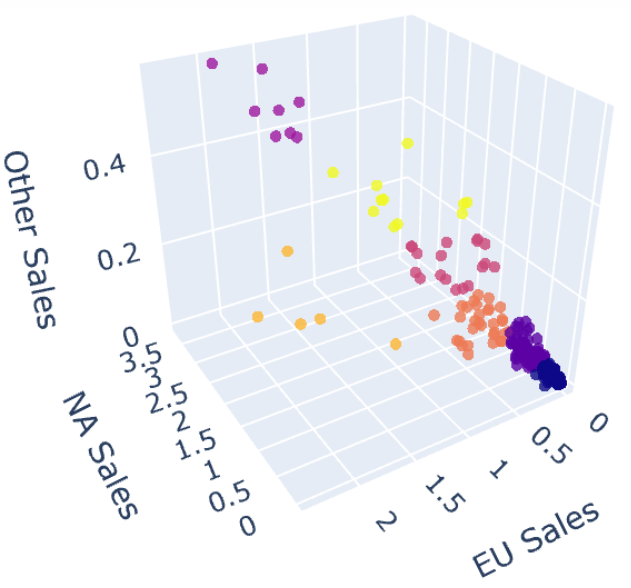
\includegraphics[width=0.8\textwidth]{img/gmm_scatter.png} 
        \caption{GMM Clusters}
        \label{fig:subim1}
    \end{subfigure}
    \begin{subfigure}{0.5\textwidth}
        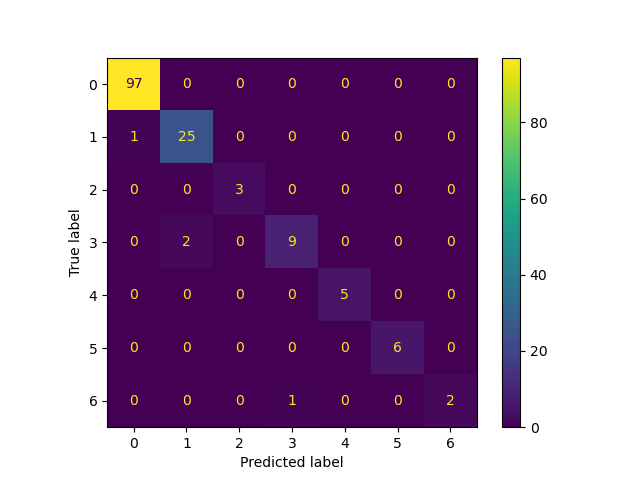
\includegraphics[width=1\textwidth]{img/confusion_matrix.png}
        \caption{RF Classifier Confusion Matrix}
        \label{fig:subim2}
    \end{subfigure}
    
    \caption{Visualisation of Clustering and Classifying Results}
    \label{fig:image2}
\end{figure}

\vspace{1cm}

\begin{figure}[h]
    \centering
    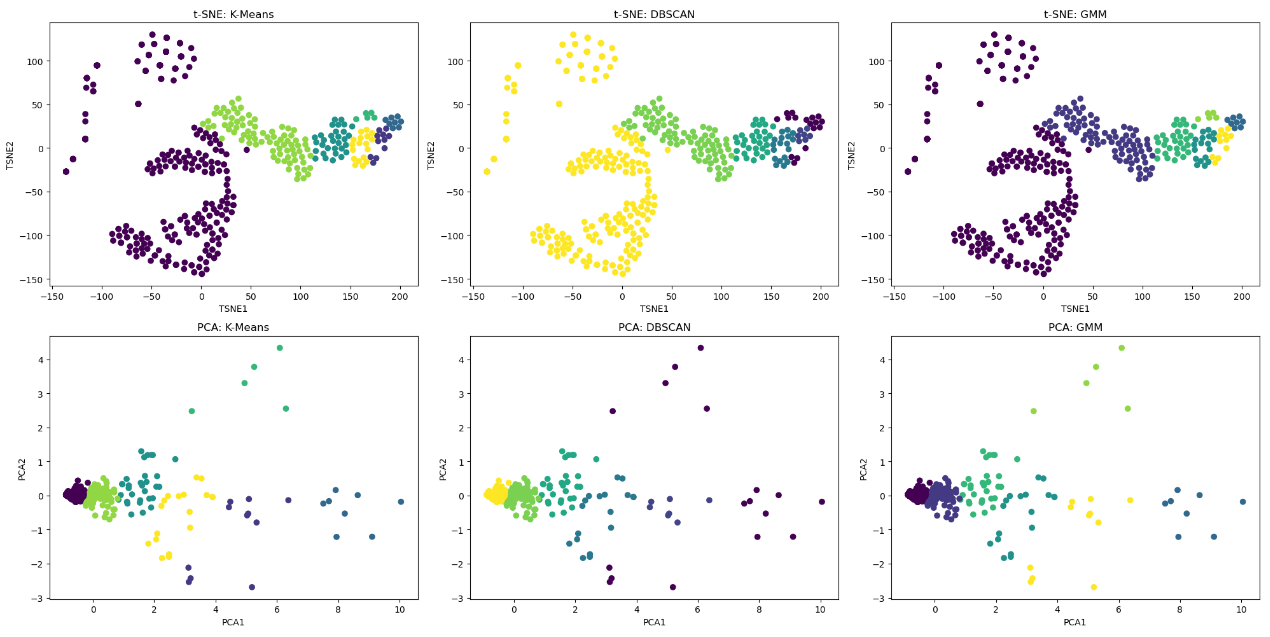
\includegraphics[width=1\textwidth]{img/dimensionality_reduction.png}
        \vspace{-2mm}
    \caption{Dimensionality Reduction for Clusters}
\end{figure}

\end{document}